\chapter{Status dos Casos de Uso}

Este capítulo apresenta o estado atual de implementação dos casos de uso definidos na Entrega~2 do projeto. O desenvolvimento do SGC adota uma abordagem incremental, priorizando os fluxos de maior impacto operacional. O protótipo funcional da interface foi desenvolvido com a stack definida na arquitetura --- React no front-end, com integração prevista à API FastAPI e ao banco de dados PostgreSQL via Supabase.

\section{Visão Geral do Estado de Implementação}

A \autoref{tab:status-ucs} consolida a situação de cada caso de uso, classificando-o em uma das três categorias: \textbf{Funcional} (tela implementada, navegação ativa e dados de demonstração integrados), \textbf{Parcial} (funcionalidade presente como subcomponente de outro módulo) ou \textbf{Planejado} (escopo definido, implementação não iniciada).

\renewcommand{\arraystretch}{1.3}
\begin{table}[H]
\centering
\small
\begin{tabularx}{\textwidth}{|p{1.2cm}|p{5.2cm}|p{2.8cm}|X|}
\hline
\textbf{ID} & \textbf{Caso de Uso} & \textbf{Status} & \textbf{Observação} \\ \hline
UC01 & Gerenciar Cadastro de Pacientes   & Funcional & Tabela de pacientes com busca por nome/CPF, indicadores de status, formulário de cadastro e edição, e ação de inativação. \\ \hline
UC02 & Gerenciar Agenda de Consultas     & Funcional & Calendário semanal com filtro por profissional, codificação visual por status e botão de novo agendamento. \\ \hline
UC03 & Configurar Grade de Horários      & Planejado           & Definido no escopo; implementação prevista para fase seguinte. \\ \hline
UC04 & Realizar Atendimento Clínico      & Funcional & Prontuário eletrônico com sinais vitais, histórico de atendimentos por CID, anamnese estruturada (queixa principal, HDA, conduta) e abas de receita e documentos. \\ \hline
UC05 & Emitir Prescrição Médica          & Parcial             & Aba ``Receita'' presente no módulo de Prontuário com lista de medicamentos e geração de PDF. \\ \hline
UC06 & Dispensar Medicamentos            & Planejado           & Definido no escopo; fluxo de dispensação previsto para integração com o módulo de farmácia. \\ \hline
UC07 & Gerenciar Estoque Farmacêutico    & Funcional & Inventário com código, lote, quantidade, mínimo, validade e alertas automáticos de ruptura. \\ \hline
UC08 & Faturar Atendimento               & Planejado           & Definido no escopo; módulo financeiro previsto para fase seguinte. \\ \hline
UC09 & Administrar Usuários e Permissões & Parcial             & Autenticação com seleção de perfil RBAC implementada na tela de login; gestão administrativa não implementada. \\ \hline
UC10 & Gerenciar Salas e Equipamentos    & Planejado           & Definido no escopo; módulo de infraestrutura previsto para fase seguinte. \\ \hline
\end{tabularx}
\caption{Status de implementação dos casos de uso do SGC}
\label{tab:status-ucs}
\end{table}

\section{Casos de Uso Funcionais}

As seções a seguir apresentam as telas implementadas para os três casos de uso destacados neste incremento, com descrição das funcionalidades disponíveis em cada módulo.

%%────────────────────────────────────────────────
\subsection{UC01 --- Gerenciar Cadastro de Pacientes}

O módulo de Cadastro de Pacientes exibe três indicadores no topo: total cadastrado, ativos e inativos. A tabela lista cada paciente com nome, CPF, data de nascimento, telefone, convênio e status colorido (\textbf{Ativo} em verde, \textbf{Inativo} em cinza), com ações de \textbf{edição} e \textbf{inativação}. O botão ``Novo paciente'' abre formulário inline com validação de CPF duplicado.

\begin{figure}[htbp]
\centering
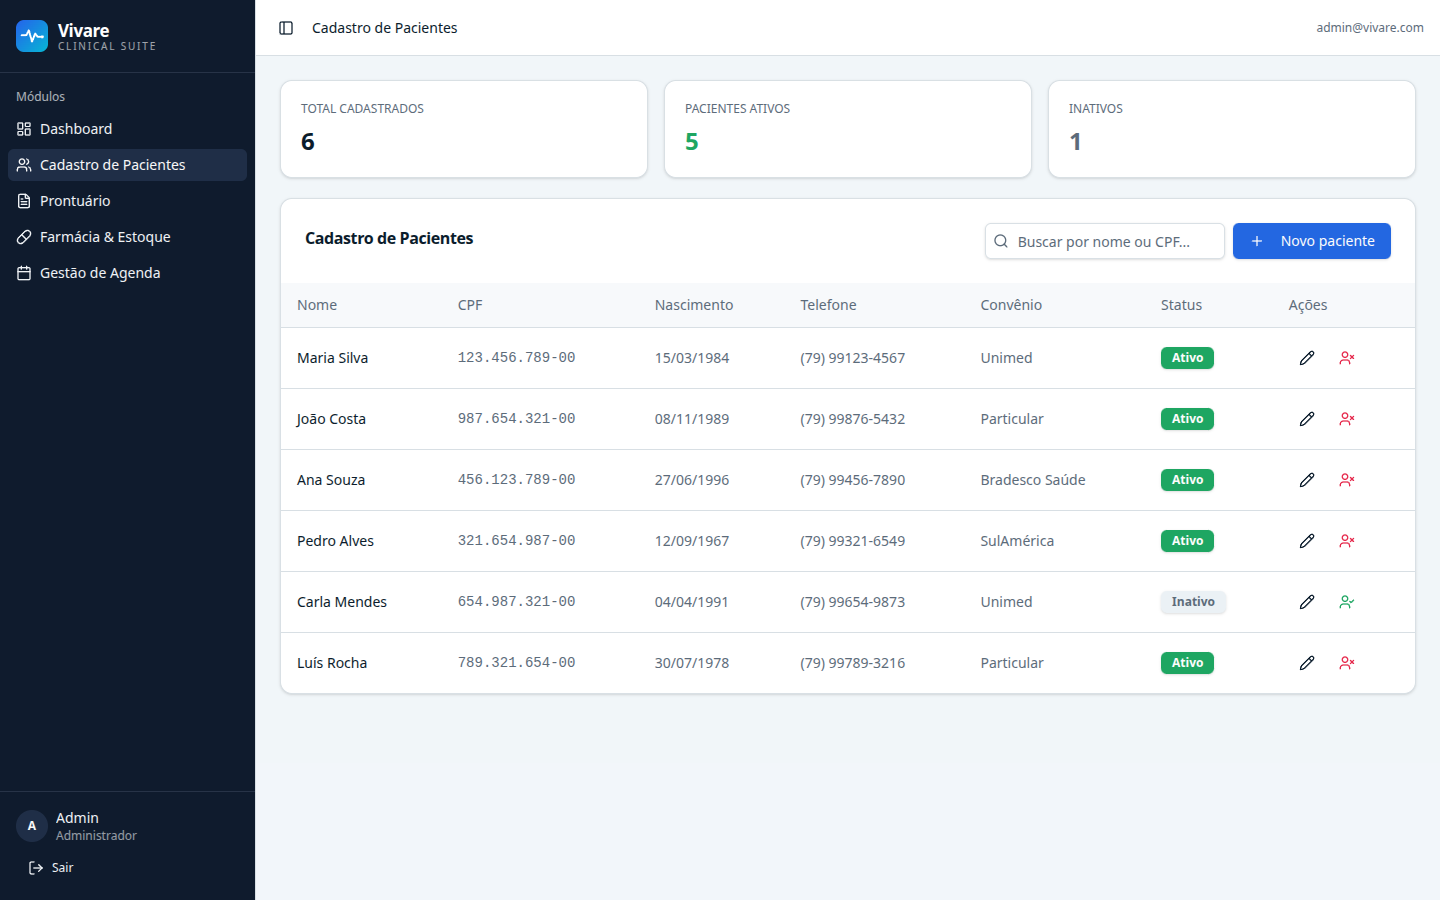
\includegraphics[width=\textwidth,height=0.37\textheight,keepaspectratio]{Imagens/cap6-tela-pacientes.png}
\caption{Tela do módulo Cadastro de Pacientes --- UC01}
\label{fig:cap6-pacientes}
\end{figure}

%%────────────────────────────────────────────────
\subsection{UC02 --- Gerenciar Agenda de Consultas}

O módulo de Gestão de Agenda implementa visão semanal com navegação entre semanas e filtro por profissional. Cada compromisso exibe nome do paciente, médico responsável e código de cor por status: \textbf{confirmado} (azul), \textbf{em atendimento} (verde), \textbf{aguardando} (cinza) e \textbf{conflito} (vermelho). O botão ``Novo agendamento'' está disponível na barra de controles.

\begin{figure}[htbp]
\centering
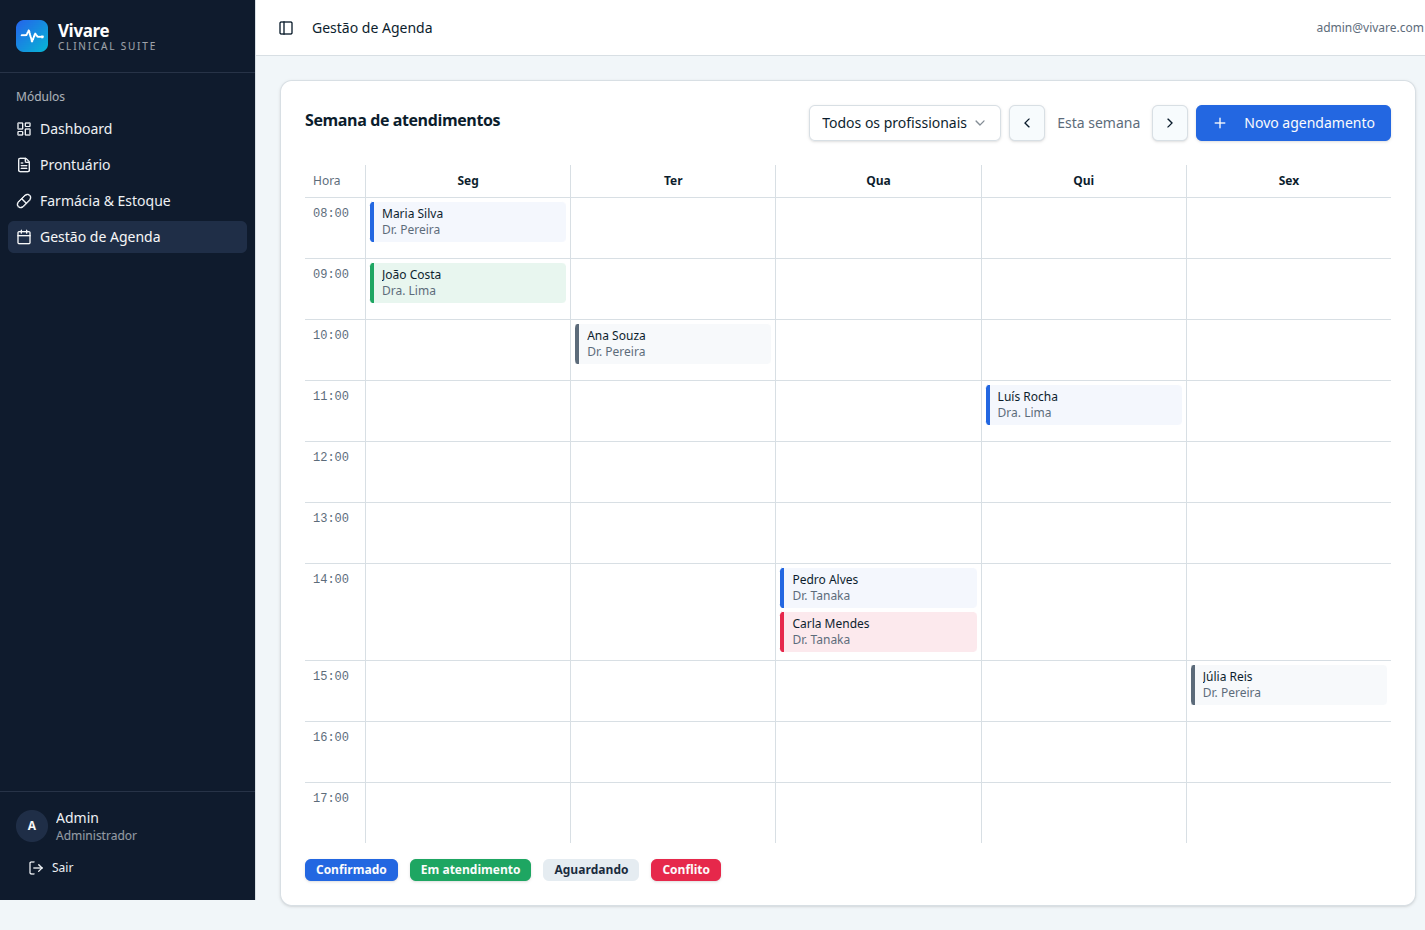
\includegraphics[width=\textwidth,height=0.37\textheight,keepaspectratio]{Imagens/cap6-tela-agenda.png}
\caption{Tela do módulo Gestão de Agenda --- UC02}
\label{fig:cap6-agenda}
\end{figure}

%%────────────────────────────────────────────────
\subsection{UC04 --- Realizar Atendimento Clínico}

O módulo de Prontuário Eletrônico apresenta busca de pacientes em tempo real. Ao selecionar um paciente, o painel exibe: dados cadastrais com tipo sanguíneo e alergias em destaque, seis sinais vitais (PA, FC, temperatura, SpO\textsubscript{2}, peso e IMC) e histórico de atendimentos anteriores com data, CID, diagnóstico, médico e tipo de visita. A evolução clínica é registrada em campos estruturados de \textbf{queixa principal}, \textbf{HDA} e \textbf{conduta}, com abas de \textbf{Receita} e \textbf{Documentos}.

\begin{figure}[htbp]
\centering
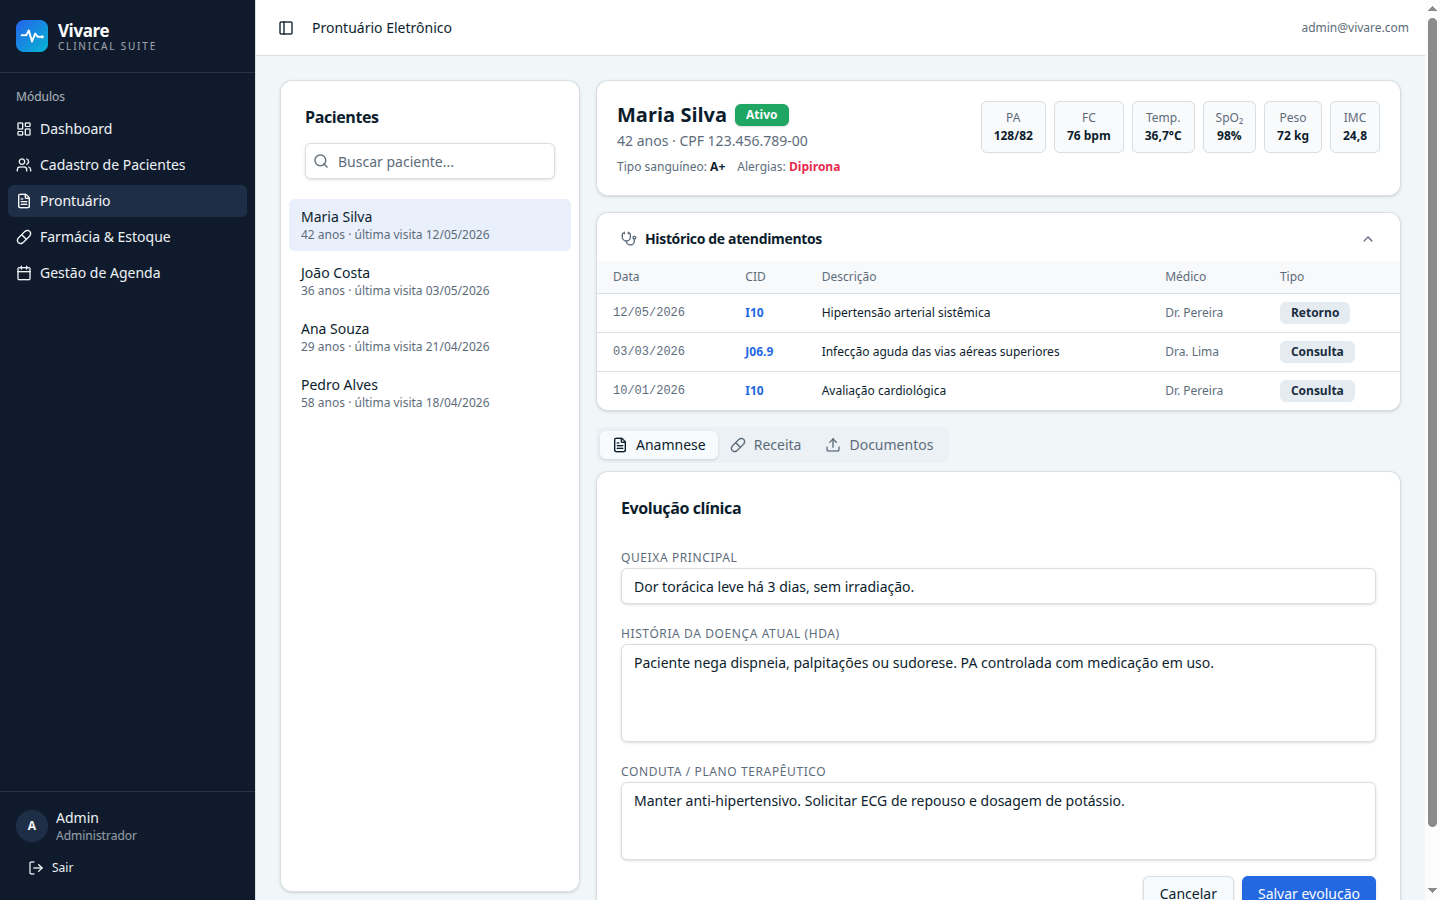
\includegraphics[width=\textwidth,height=0.37\textheight,keepaspectratio]{Imagens/cap6-tela-prontuario.png}
\caption{Tela do módulo Prontuário Eletrônico --- UC04}
\label{fig:cap6-prontuario}
\end{figure}

\section{Considerações sobre os Próximos Incrementos}

Os casos de uso classificados como \textbf{Planejado} (UC03, UC06, UC08 e UC10) têm seus fluxos completamente especificados na Entrega~2 e suas entidades mapeadas no modelo objeto-relacional deste documento. A prioridade para o próximo incremento é UC06 (Dispensar Medicamentos), que complementa diretamente o módulo de farmácia já disponível, e UC08 (Faturar Atendimento), cujos dados de entrada já são produzidos pelos módulos de agenda e prontuário implementados.
